\documentclass{article}
\usepackage[utf8]{inputenc}
\title{Project Proposal}
\author{Benjamin E Sher}
\date{October 2018}
\usepackage{natbib}
\usepackage{graphicx}
\begin{document}
\maketitle
\section{Introduction}
I am going to use C to build a video game based on the hit arcade game
Q*BERT.\@ This game will be a platformer/puzzle game using traditional
side-scrolling methods and techniques.
\begin{figure}[h!]
\centering
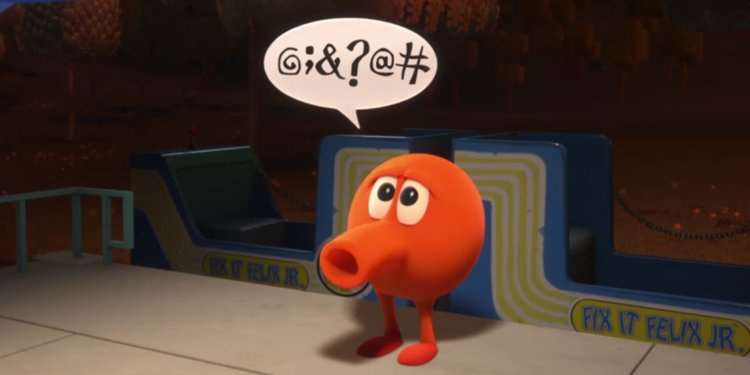
\includegraphics[scale=.25]{qbert}
\caption{Q*BERT}
\end{figure}
This Little guy will be converted to a small ASCII avatar:
\begin{figure}[h!]
\centering
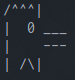
\includegraphics[scale=1]{acq}
\caption{Q*BERT ASCII}
\end{figure}
And then made to interact and move within a ASCII environment, hostile or
otherwise. Other characters from the original game will appear, such as the
snake as well as some of the classic obstacles like green balls. This will all
lead to a playing expirence hopefully similar to the SMB3 feel.\@
\newline
\newline
\section{Features}
1. Object Collision - 15 points
\newline
2. Hit detection - 15 points
\newline
3. Random spawns of enemies and obstacles - 30 points
\newline
4. Different and random enemy pathing - 40 points
\newline
5. Hidden retro throwback level (Bonus) - 30 points
\newline
\section{Mission Statement}
`'To make a fun and retro styled Q*BERT sidescrolling game with fun puzzles and
enemies''
\end{document}
